\documentclass[a4paper]{jpconf}
\usepackage{graphicx}
\usepackage{hyperref}
\usepackage{listings}
\usepackage{color}
\usepackage{enumitem}
%\lstloadlanguages{javascript,xml}
%\pagenumbering{roman}

\definecolor{gray}{rgb}{0.4,0.4,0.4}
\definecolor{darkblue}{rgb}{0.0,0.0,0.6}
\definecolor{cyan}{rgb}{0.0,0.6,0.6}

\lstset{
  language = XML,
  basicstyle=\ttfamily,
  columns=fullflexible,
  showstringspaces=false,
  commentstyle=\color{gray}\upshape
}

\lstdefinelanguage{XML}
{
  morestring=[b]",
  morestring=[s]{>}{<},
  morecomment=[s]{<?}{?>},
  stringstyle=\color{black},
  identifierstyle=\color{darkblue},
  keywordstyle=\color{cyan},
  morekeywords={xmlns,version,type}% list your attributes here
}

\lstset { %
    language=C++,
  %  backgroundcolor=\color{black!5}, % set backgroundcolor
    basicstyle=\footnotesize% basic font setting
}

%
\lstdefinelanguage{JavaScript}{
  keywords={typeof, new, true, false, catch, function, return, null, catch, switch, var, if, in, while, do, else, case, break},
  keywordstyle=\color{blue}\bfseries,
  ndkeywords={class, export, boolean, throw, implements, import, this},
  ndkeywordstyle=\color{black}\bfseries,
  identifierstyle=\color{black},
  sensitive=false,
  comment=[l]{//},
  morecomment=[s]{/*}{*/},
  commentstyle=\color{green}\ttfamily,
  stringstyle=\color{red}\ttfamily,
  morestring=[b]',
  morestring=[b]"
}

\lstset{
   language=JavaScript,
  % backgroundcolor=\color{lightgray},
   extendedchars=true,
   basicstyle=\footnotesize\ttfamily,
   showstringspaces=false,
   showspaces=false,
   numbers=left,
   numberstyle=\footnotesize,
   numbersep=9pt,
   tabsize=2,
   breaklines=true,
   showtabs=false,
   captionpos=b
}

\begin{document}
 % \title{Preparing a paper using \LaTeXe\ for publication in \jpcs}
\title{New ROOT graphics language}

\author{Iliana Betsou, Serguei Linev, Bertrand Bellenot, Olivier Couet}

\address{Production Editor, \jpcs, \iopp, Dirac House, Temple Back, Bristol BS1~6BE, UK}

\ead{iliana.betsou@cern.ch, s.linev@gsi.de, bertrand.bellenot@cern.ch, olivier.couet@cern.ch}

\begin{abstract}
In the context of ROOT7, the graphics system is completely redefined. Based on client server architecture and with the use of modern C++ and JavaScript, ROOT7 provides a new web based graphics system. The new concepts of ROOT7 can be displayed directly in the browsers using the new classes for opening a new web window, communicate with the server and exchange data between front and back end and JavaScript ROOT (JSROOT).
\end{abstract}

\section{Introduction}
\href{https://root.cern.ch/}{ROOT}~\cite{root} exists for more than two decades and from the beginning, it has its own graphics system. This graphics system~\cite{Antcheva:2011zz} used the most popular technologies at that time, like OpenGL and X11. With the rapid development of technology of the last years and the high turn on the web technology, it was time for changing the whole graphics system. The new ROOT7's graphics library in ROOT, with the use of modern C++ and web based architecture, redefine completely ROOT graphics (Figure 1) and introduce a new web based environment.
\\
% \begin{figure}[h]
% \includegraphics[width=26pc]{WebEve1.eps}\hspace{2pc}%
% \begin{minipage}[b]{14pc}\caption{\label{label}The new version of web Event Visualization Environment (EVE)}
% \end{minipage}
% \end{figure}
\begin{figure}[h]
  \begin{center}
    \includegraphics[width=15pc]{alice.eps}\hspace{2pc}%
  \end{center}
\centering
\begin{minipage}[b]{25pc}\caption{\label{label}Tracks and hits combined with ALICE detector}
\end{minipage}
\end{figure}


\section{Objectives of the new version}

\subsection{Need of new graphics}
In the current version of ROOT6~\cite{root6}, there were some problems:
\begin{itemize}
  \item the current Graphical User Interface (GUI) is very {OS-specific}, originally based on X11
  \item using OpenGL with remote X11 is not very efficient
  \item X11 is no longer supported on MacOS and the only way to use it is through XQuartz~\cite{x11}
  \item ROOT6 is single-threaded
  \item long term maintenance problems
\end{itemize}

\subsection{Goals of the new Version}
Fixing these problems is the main goal of the new version of ROOT. The new system is based on widely used technologies like SVG and WebGL, which are supported by a large community. The main goal is to have a remote/web GUI with some specific characteristics. It has to be portable and to support remote displays and multiple views. It is also very important to be multi threaded and to support any new future platform.

\section{ROOT7}

The answer to all the above is \href{https://root.cern.ch/root-7}{ROOT7}~\cite{root7}. A local application, which uses web technologies and it is able to run in a web browser. ROOT7 is web based, easy to use with a modern and clear layout.
%
A web based application (as ROOT7) is a client/server computer application (Figure 2), where the client and its user interface run directly on the browser. ROOT7 consists of \href{https://root.cern.ch/js/}{JSROOT}~\cite{jsroot} and implements a \href{https://en.wikipedia.org/wiki/Model%E2%80%93view%E2%80%93controller}{Model-View-Controller(MVC)}~\cite{mvc} architecture. The server side is written in C++ and the client side in JavaScript.
The most important classes are THttpServer~\cite{http} which is responsible for the communication between the different parts and TBufferJSON~\cite{buffer} which is responsible for the I/O. The GUI framework is \textit{OpenUI5}~\cite{openui} created by \href{https://www.sap.com/index.html}{SAP}.

\begin{figure}[h]
  \begin{center}
    \includegraphics[width=25pc]{client-server.eps}\hspace{2pc}%
  \end{center}
  \centering
\begin{minipage}[b]{20pc}\caption{\label{label}Client Server model}
\end{minipage}
\end{figure}

\subsection{JSROOT}

\href{https://github.com/root-project/jsroot/}{JSROOT} is being developed since 2012 and is responsible for displaying the ROOT objects in web browsers using JavaScript~\cite{jsroot}. The displayed objects can be manipulated directly in the web browser. It can read binary data (including \href{https://root.cern.ch/doc/master/classTTree.html}{TTree}) and uses the ROOT JSON format. JSROOT is also used by the ROOT jupyter interface.


\subsection{THttpServer}

\href{https://github.com/root-project/jsroot/blob/master/docs/HttpServer.md}{THttpServer} is one of the most important components~\cite{http}. It gives HTTP access to run ROOT application and it is responsible for the execution of commands and methods. With THttpServer and JSROOT, it is possible to visualize ROOT objects. The communication is achieved via WebSockets protocol, which is bidirectional and supports binary data. WebSocket is a communication protocol providing full-duplex communication channels over a single TCP connection.

\subsection{TBufferJSON}

\href{https://root.cern.ch/doc/master/classTBufferJSON.html}{TBufferJSON} can converts any streamable C++ object to JSON and vise versa~\cite{buffer}; also custom streamers can be supported. With the use of TBufferJSON the data exchange between C++ server and JavaScript client is simple. Real ROOT I/O remains fully on the server side.

\subsection{OpenUI5}
The design of the GUI layout is based on \textit{\href{https://openui5.hana.ondemand.com/}{OpenUI5}}~\cite{openui} which is a JavaScript UI library consisting of a really large number of UI controls. \textit{OpenUI5} implements the MVC~\cite{mvc} architecture, which separates out the application logic into three separate parts:
\begin{itemize}
  \item The Model component which is the central component and contains the application's dynamic data.
  \item The View component is the final output that ends up in the user's browser and defines how the application's data should be displayed.
  \item The Controller component receives inputs and contains the logic that updates the model or the view, depending on the inputs.
\end{itemize}

\subsection{RWebWindow Class}
The RWebWindow~\cite{rweb} class is a server-side entity in new ROOT window management. It displays windows in the web browser and manage multiple connections with the clients. This class transfers the data from and to the clients. It also supports the batch mode (by using \textit{headless} mode).

 \subsection{Graphics Model}

 The new graphics model is independent from any local graphics backend. It allows remote display on all kind of devices. The JavaScript rendering is able to be performed in a local canvas.

\section{Concepts of ROOT7}
There are three main concepts in ROOT7:
\begin{enumerate}[label=\alph*)]
  \item The \textit{Pad} is a base entity containing the list of graphics objects to be drawn and is implemented by \textit{\href{https://root.cern.ch/doc/master/classROOT_1_1Experimental_1_1RPad.html}{RPad}} class.
  \item The \textit{Canvas}, the window's topmost pad, implemented by \textit{\href{https://root.cern.ch/doc/master/classROOT_1_1Experimental_1_1RCanvas.html}{RCanvas}}.
  \item The Drawable entity. Drawable can be anything that can be drawn on a pad. Each drawable entity has a \textbf{GetDrawable} method and is implemented in \textit{\href{https://root.cern.ch/doc/master/classROOT_1_1Experimental_1_1RDrawable.html}{RDrawable}} class.
\end{enumerate}

% \begin{figure}[h]
% 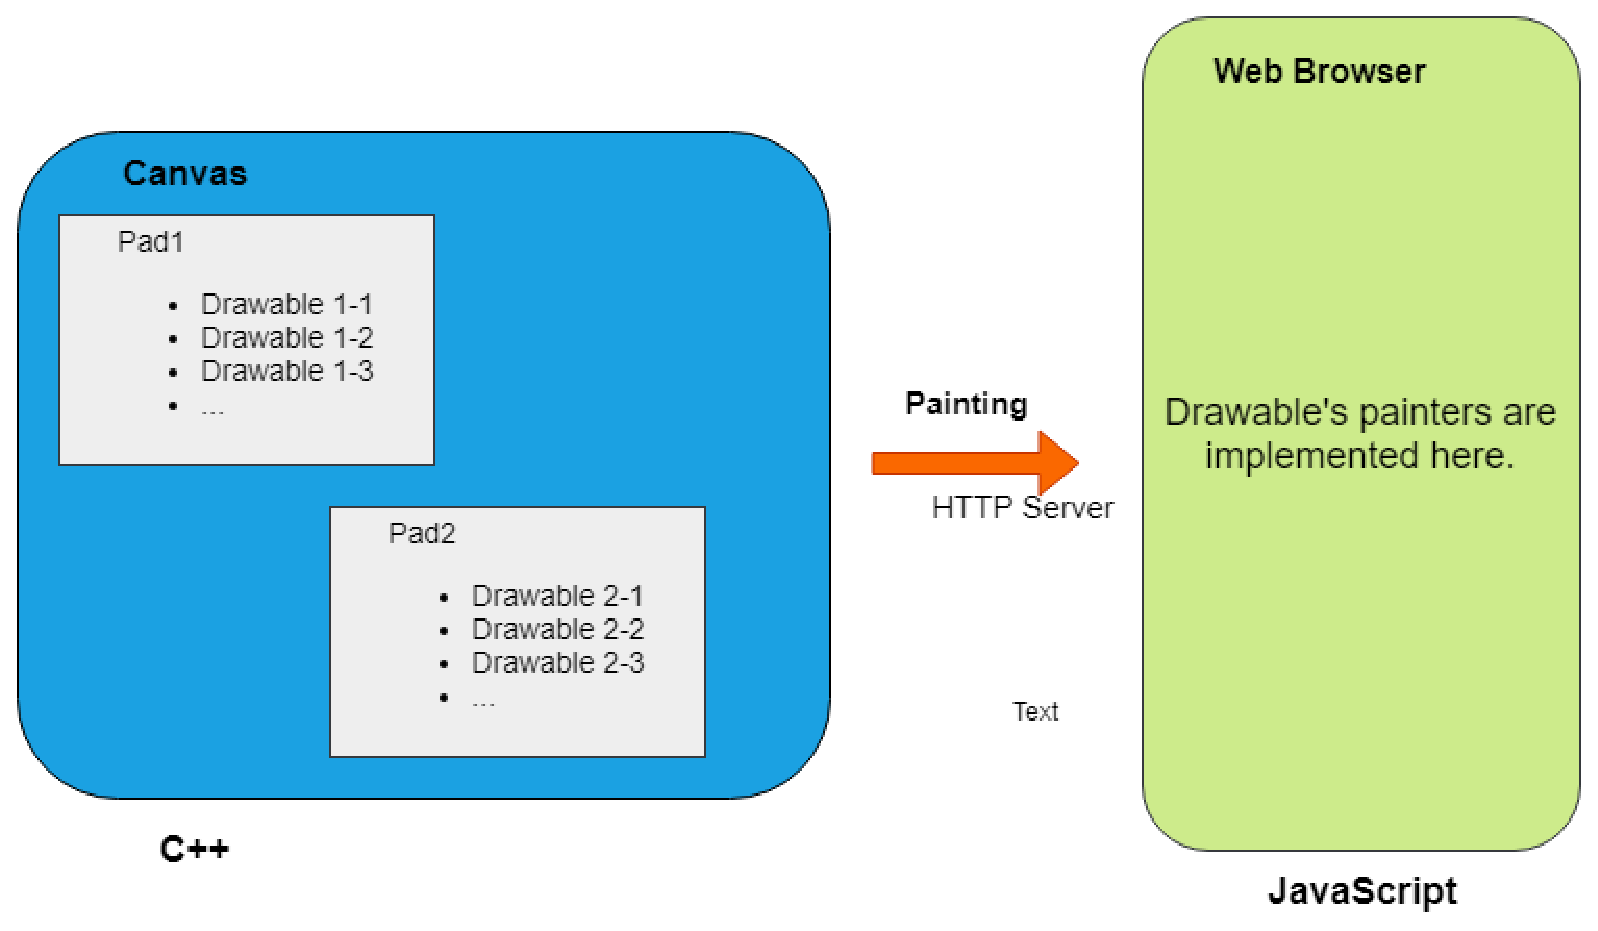
\includegraphics[width=26pc]{BasicConcepts.eps}\hspace{2pc}%
% \begin{minipage}[b]{14pc}\caption{\label{label}Basic Concepts of ROOT7}
% \end{minipage}
% \end{figure}

\section{Batch Output}
In the current state of ROOT, there are two main kinds of batch output images:
\begin{itemize}
  \item \textbf{Vector graphics output} (like PDF and SVG) which is implemented by native ROOT classes
  \item \textbf{Bitmap output} (like PNG and JPEG) which is implemented natively on top of libAfterImage
\end{itemize}

\noindent
In the new ROOT7, one of the main goals is not rely on any dedicated ROOT libraries. The best way to achieve this is to use the \textit{}{Headless mode} of the web browsers when complete HTML/JavaScript/SVG/WebGL code can work without any real screen display. This mode is able to generate the appropriate output.

\section{Example: Fit Panel}

The new version of \href{https://root.cern.ch/fit-panel}{Fit panel} is a simple example of the use of all the aboves, in particular the \textit{OpenUI5} environment.

\begin{figure}[h]
  \centering
\begin{minipage}{14pc}
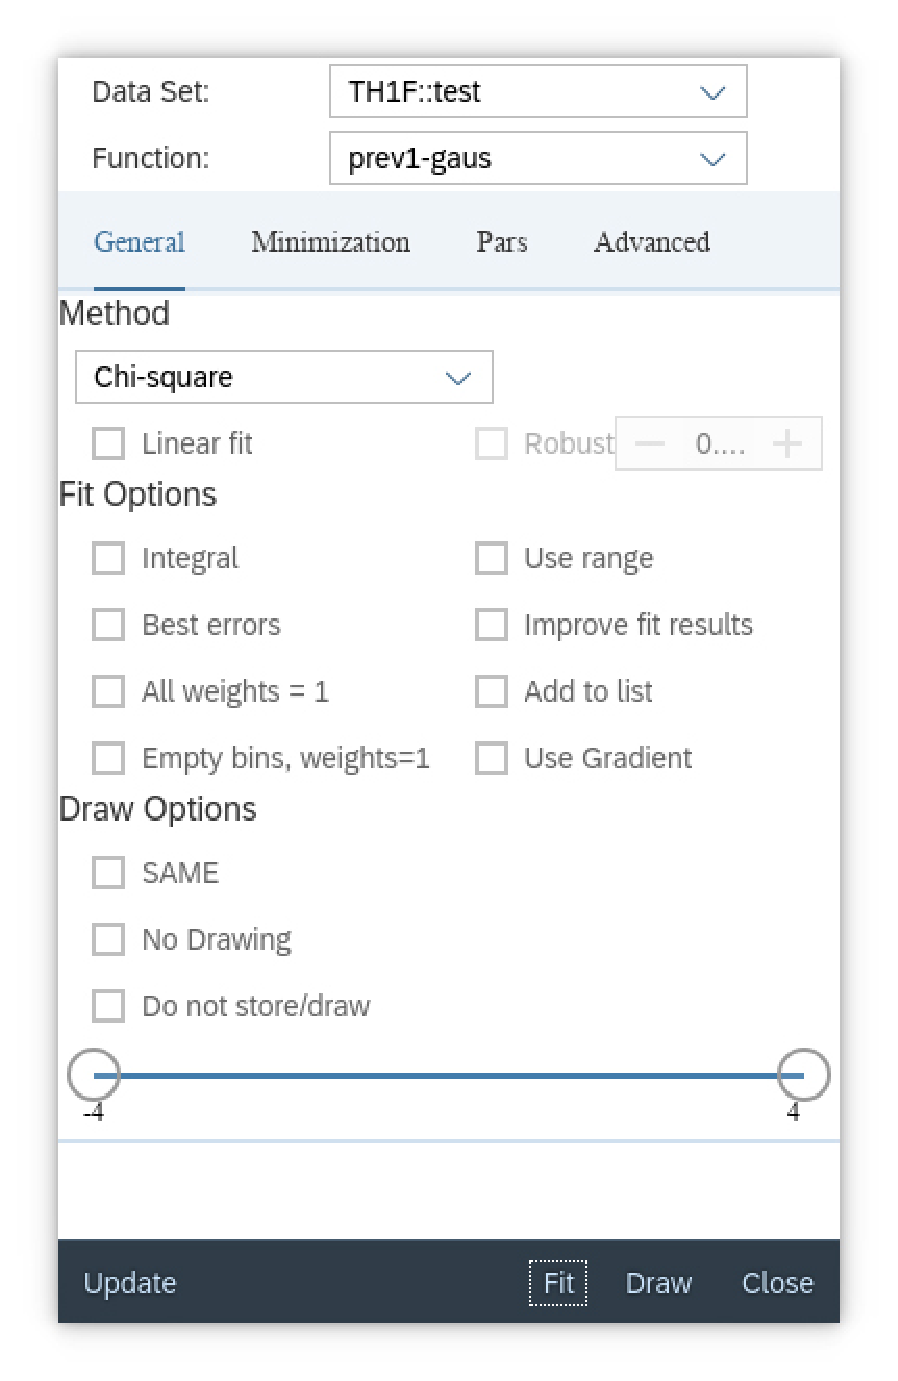
\includegraphics[width=16pc]{rfitpanel1.eps}
\caption{\label{label}ROOT7 version of fit panel}
\end{minipage}\hspace{2pc}%
\begin{minipage}{14pc}
\includegraphics[width=15pc]{oldPanel.eps}
\caption{\label{label}ROOT6 version of fit panel}
\end{minipage}
\end{figure}

The fit panel is a user interface based on a client/server model and it runs directly in the browser. The layout is based on \textit{OpenUI5} framework. It uses all the power of ROOT fitting tools to interactively fit histograms, using predefined functions (such as Gaus, Exponential, Polynomial)  or a function defined by the user. The user is able to choose between several options. There are options for different ROOT libraries and minimization methods along with a lot of fit and draw options as well as specific range selector to define the range of the histogram to be fit.

In fit panel there are a lot of different UI controls, some of them with static values and some other with dynamic values provided by ROOT. A small but indicative example of how the fit panel works, is the creation of a dynamic \textit{ComboBox}.
The first step is the creation of C++, which can represent data for single item in \textit{OpenUI5} \textit{ComboBox}.
\\
\begin{lstlisting}[language=C++]
/// Generic item for ui5 ComboBox
struct RComboBoxItem {
  std::string key;
  std::string value;
  RComboBoxItem() = default;
  RComboBoxItem(const std::string &_key, const std::string &_value) : key(_key), value(_value) {}
};
\end{lstlisting}
\noindent
Then there is a model object which should contains all necessary elements to configure \textit{OpenUI5} \textit{ComboBox} .

\begin{lstlisting}[language=C++]
struct RFitPanelModel {
  std::vector<RComboBoxItem> fItems;
  std::string fSelected;
}
\end{lstlisting}
\noindent
It includes vector of items \textit{fItems} and selected element \textit{fSelected}.
The next step is to fill this structure with available values and send it to the client as JSON, using TBufferJSON class for transformation:

\begin{lstlisting}[language=C++]
  RFitPanelModel model;
  model.fItems = {{"id0", "value0"}, {"id1", "value1"}, {"id2", "value2"}};
  model.fSelected = "id1";

  auto json = TBufferJSON::ToJSON(&model);

  fWindow->Send(fConnId, "MODEL:"s + json.Data());
\end{lstlisting}

\noindent Produced JSON code:

\begin{lstlisting}[language=XML]
  {
     "_typename" : "RFitPanelModel",
     "fItems" : [{
       "_typename" : "RComboBoxItem",
       "key" : "id0",
       "value" : "value0"
     }, {
       "_typename" : "RComboBoxItem",
       "key" : "id1",
       "value" : "value1"
     }, {
       "_typename" : "RComboBoxItem",
       "key" : "id2",
       "value" : "value2"
     }],
     "fSelected" : "id1"
  }
\end{lstlisting}
\noindent
When JSON data received by the JavaScript client, it should be parsed and model object assigned to the view:

\begin{lstlisting}[language=JavaScript]
  obj = JSROOT.parse(str);
  this.getView().setModel(new JSONModel(obj));
\end{lstlisting}
\noindent
For displaying of the \textit{ComboBox} with provided data, it should be defined in the XML view files as follow:

\begin{lstlisting}[language=XML]
  <ComboBox selectedKey="{/fSelected}"
            items="{ path: '/fItems' }">
               <core:Item key="{id}" text="{text}" />
  </ComboBox>
\end{lstlisting}

\noindent
And the produced \textit{ComboBox} element can be seen in Figure 5.
\begin{figure}[h]
  \begin{center}
    \includegraphics[width=10pc]{testCombo.eps}\hspace{2pc}%
  \end{center}
  \centering
\begin{minipage}[b]{20pc}\caption{\label{label}The produced \textit{ComboBox}}
\end{minipage}
\end{figure}
\\
\noindent
Once option is selected, it should be send back to the server side in JSON format.
\begin{lstlisting}[language=JavaScript]
  var json = this.getView().getModel().getJSON();

  this.websocket.Send("MODEL:" + json);
\end{lstlisting}
\noindent
The final step is decoding such JSON data on C++ and processing corresponding ROOT functions:

\begin{lstlisting}[language=C++]
  auto model = TBufferJSON::FromJSON<RFitPanelModel>(json);

  if (model.fSelected == "id0"){
    // do first branch
  }
  if (model.fSelected == "id1"){
    // do second branch
  }
  if (model.fSelected == "id2"){
    // do third branch
  }
\end{lstlisting}
\noindent
The operation can be repeated many items.


\section{Conclusion}

To summarize all the above, the ROOT7 graphics system is based on new technologies like (SVG/HTML/WebGL). It implements a client/server model, where the client side is written in JavaScript and the server side in C++. The batch output will not rely anymore on any native ROOT libraries and this is achieved with the use of browser's headless mode.




\section{References}
\bibliography{iopart-num}

\end{document}
